% Options for packages loaded elsewhere
\PassOptionsToPackage{unicode}{hyperref}
\PassOptionsToPackage{hyphens}{url}
%
\documentclass[
]{article}
\usepackage{lmodern}
\usepackage{amssymb,amsmath}
\usepackage{ifxetex,ifluatex}
\ifnum 0\ifxetex 1\fi\ifluatex 1\fi=0 % if pdftex
  \usepackage[T1]{fontenc}
  \usepackage[utf8]{inputenc}
  \usepackage{textcomp} % provide euro and other symbols
\else % if luatex or xetex
  \usepackage{unicode-math}
  \defaultfontfeatures{Scale=MatchLowercase}
  \defaultfontfeatures[\rmfamily]{Ligatures=TeX,Scale=1}
\fi
% Use upquote if available, for straight quotes in verbatim environments
\IfFileExists{upquote.sty}{\usepackage{upquote}}{}
\IfFileExists{microtype.sty}{% use microtype if available
  \usepackage[]{microtype}
  \UseMicrotypeSet[protrusion]{basicmath} % disable protrusion for tt fonts
}{}
\makeatletter
\@ifundefined{KOMAClassName}{% if non-KOMA class
  \IfFileExists{parskip.sty}{%
    \usepackage{parskip}
  }{% else
    \setlength{\parindent}{0pt}
    \setlength{\parskip}{6pt plus 2pt minus 1pt}}
}{% if KOMA class
  \KOMAoptions{parskip=half}}
\makeatother
\usepackage{xcolor}
\IfFileExists{xurl.sty}{\usepackage{xurl}}{} % add URL line breaks if available
\IfFileExists{bookmark.sty}{\usepackage{bookmark}}{\usepackage{hyperref}}
\hypersetup{
  pdftitle={Final Project},
  pdfauthor={Han},
  hidelinks,
  pdfcreator={LaTeX via pandoc}}
\urlstyle{same} % disable monospaced font for URLs
\usepackage[margin=1in]{geometry}
\usepackage{color}
\usepackage{fancyvrb}
\newcommand{\VerbBar}{|}
\newcommand{\VERB}{\Verb[commandchars=\\\{\}]}
\DefineVerbatimEnvironment{Highlighting}{Verbatim}{commandchars=\\\{\}}
% Add ',fontsize=\small' for more characters per line
\usepackage{framed}
\definecolor{shadecolor}{RGB}{248,248,248}
\newenvironment{Shaded}{\begin{snugshade}}{\end{snugshade}}
\newcommand{\AlertTok}[1]{\textcolor[rgb]{0.94,0.16,0.16}{#1}}
\newcommand{\AnnotationTok}[1]{\textcolor[rgb]{0.56,0.35,0.01}{\textbf{\textit{#1}}}}
\newcommand{\AttributeTok}[1]{\textcolor[rgb]{0.77,0.63,0.00}{#1}}
\newcommand{\BaseNTok}[1]{\textcolor[rgb]{0.00,0.00,0.81}{#1}}
\newcommand{\BuiltInTok}[1]{#1}
\newcommand{\CharTok}[1]{\textcolor[rgb]{0.31,0.60,0.02}{#1}}
\newcommand{\CommentTok}[1]{\textcolor[rgb]{0.56,0.35,0.01}{\textit{#1}}}
\newcommand{\CommentVarTok}[1]{\textcolor[rgb]{0.56,0.35,0.01}{\textbf{\textit{#1}}}}
\newcommand{\ConstantTok}[1]{\textcolor[rgb]{0.00,0.00,0.00}{#1}}
\newcommand{\ControlFlowTok}[1]{\textcolor[rgb]{0.13,0.29,0.53}{\textbf{#1}}}
\newcommand{\DataTypeTok}[1]{\textcolor[rgb]{0.13,0.29,0.53}{#1}}
\newcommand{\DecValTok}[1]{\textcolor[rgb]{0.00,0.00,0.81}{#1}}
\newcommand{\DocumentationTok}[1]{\textcolor[rgb]{0.56,0.35,0.01}{\textbf{\textit{#1}}}}
\newcommand{\ErrorTok}[1]{\textcolor[rgb]{0.64,0.00,0.00}{\textbf{#1}}}
\newcommand{\ExtensionTok}[1]{#1}
\newcommand{\FloatTok}[1]{\textcolor[rgb]{0.00,0.00,0.81}{#1}}
\newcommand{\FunctionTok}[1]{\textcolor[rgb]{0.00,0.00,0.00}{#1}}
\newcommand{\ImportTok}[1]{#1}
\newcommand{\InformationTok}[1]{\textcolor[rgb]{0.56,0.35,0.01}{\textbf{\textit{#1}}}}
\newcommand{\KeywordTok}[1]{\textcolor[rgb]{0.13,0.29,0.53}{\textbf{#1}}}
\newcommand{\NormalTok}[1]{#1}
\newcommand{\OperatorTok}[1]{\textcolor[rgb]{0.81,0.36,0.00}{\textbf{#1}}}
\newcommand{\OtherTok}[1]{\textcolor[rgb]{0.56,0.35,0.01}{#1}}
\newcommand{\PreprocessorTok}[1]{\textcolor[rgb]{0.56,0.35,0.01}{\textit{#1}}}
\newcommand{\RegionMarkerTok}[1]{#1}
\newcommand{\SpecialCharTok}[1]{\textcolor[rgb]{0.00,0.00,0.00}{#1}}
\newcommand{\SpecialStringTok}[1]{\textcolor[rgb]{0.31,0.60,0.02}{#1}}
\newcommand{\StringTok}[1]{\textcolor[rgb]{0.31,0.60,0.02}{#1}}
\newcommand{\VariableTok}[1]{\textcolor[rgb]{0.00,0.00,0.00}{#1}}
\newcommand{\VerbatimStringTok}[1]{\textcolor[rgb]{0.31,0.60,0.02}{#1}}
\newcommand{\WarningTok}[1]{\textcolor[rgb]{0.56,0.35,0.01}{\textbf{\textit{#1}}}}
\usepackage{graphicx,grffile}
\makeatletter
\def\maxwidth{\ifdim\Gin@nat@width>\linewidth\linewidth\else\Gin@nat@width\fi}
\def\maxheight{\ifdim\Gin@nat@height>\textheight\textheight\else\Gin@nat@height\fi}
\makeatother
% Scale images if necessary, so that they will not overflow the page
% margins by default, and it is still possible to overwrite the defaults
% using explicit options in \includegraphics[width, height, ...]{}
\setkeys{Gin}{width=\maxwidth,height=\maxheight,keepaspectratio}
% Set default figure placement to htbp
\makeatletter
\def\fps@figure{htbp}
\makeatother
\setlength{\emergencystretch}{3em} % prevent overfull lines
\providecommand{\tightlist}{%
  \setlength{\itemsep}{0pt}\setlength{\parskip}{0pt}}
\setcounter{secnumdepth}{-\maxdimen} % remove section numbering
\usepackage{booktabs}
\usepackage{longtable}
\usepackage{array}
\usepackage{multirow}
\usepackage{wrapfig}
\usepackage{float}
\usepackage{colortbl}
\usepackage{pdflscape}
\usepackage{tabu}
\usepackage{threeparttable}
\usepackage{threeparttablex}
\usepackage[normalem]{ulem}
\usepackage{makecell}
\usepackage{xcolor}

\title{Final Project}
\author{Han}
\date{4/13/2021}

\begin{document}
\maketitle

\hypertarget{repeated-exposure-effects-on-global-precedence}{%
\section{Repeated exposure effects on Global
Precedence}\label{repeated-exposure-effects-on-global-precedence}}

\hypertarget{introduction}{%
\subsection{Introduction}\label{introduction}}

This study aimed to test the endurance of global level influence on
local level processing. Research has shown that an object can have at
least two levels of information; the global level, or the large form, of
an object can influence how the local level, or detailed components, of
the object is visually processed. When the two levels are congruent
(consistent information between the two levels), global information can
facilitate local information processing; however, when incongruent
(inconsistent information between the two levels), global information
can impede local information processing, leading to slower response
times. This is called `global interference' and is derived from the
`congruency' effect that is calculated from comparisons between
performance with congruent stimuli vs.~performance with incongruent
stimuli.

The current literature presents inconsistent findings on whether
attention can reduce global level influence during local level
processing. To examine this, studies have utilized repeated presentation
paradigms that involve multiple presentations of a compound stimulus
(objects with a global and local level of perception) and manipulate the
level that participants must attend to for future presentations. For
example, participants may be directed to look for a target (letter
``A'') within a given compound stimulus. The level that contains the
letter ``A'' will be the last level that participants attend to for the
current stimulus and the first level that participants attend to for the
following stimulus. This is an important facet of repeated presentation
paradigms such that it enables control over the order of level
information processing over a series of compound stimulus. Furthermore,
attentional control is seen to increase with more repetitions. In other
words, attention becomes better at suppressing irrelevant information
and facilitating relevant information processing with multiple
repetitions. However, this effect has yet to be tested with compound
stimuli. As such, it is unclear whether multiple repetitions enables
better attentional control or focus on a particular level.

\hypertarget{study-description}{%
\subsection{Study Description}\label{study-description}}

This study aims to investigate whether multiple repetitions can reduce
congruency effects. The study utilizes the repeated presentation
paradigm with three additional details. Firsly, the study involves
multiple repeated presentations through a series of 7 compound stimulus
presentations, known as a run. Run position reference a stimulus
presentation by its sequential order within the run. Secondly,
participants are directed to a specific level (global or local) before
the series of compound stimulus presentation. This enables a more
voluntary, goal-oriented attentional deployment to the given task, and
stronger establishment of level relevancy in terms of information
processing (i.e., directed level contains relevant information while
other level contains irrelevant inforamtion). Lastly, the critical data
runs in this study contained only congruent stimuli (both irrelevant and
relevant levels contained target information) and manipulated whether
and when a single incongruent stimulus (irrelvant level contained
non-target while relevant level contained target) was presented in the
run.

Critical data runs only had at most 1 incongruent stimulus within a
given run. The incongruent stimulus was presented either early in the
run (run position 2), late in the run (run position 6), or not at all to
determine whether multiple repeated presentations strengthened
attentional control. Therefore, there were three types of runs; all
congruent stimuli, incongruent at 2, and incongruent at 6. The study
looked at whether there was a change in the amount of global level
interference during local information processing between the two run
positions (2 and 6). The congruence effect (e.g., global level
interference) was calculated from reponse time (RT) comparisons between
the incongruent stimulus and congruent stimulus (only in the all
congruent runs). Notably, the target letter was always present at the
relevant level in the critical runs.

Throughout the study, the stimulus was presented for 150 msec and was
immediately followed by a blank screen. Participants were tasked to
determine target letter presence (via keyboard button press) and had a
total of 2000 msec to respond as soon as the stimulus was shown.

Planned comparisons were made to look at whether the congruence effect
was lower at position 6 than position 2. Two important planned
comparisons were the RT differences for task completion between the
congruent and incongruent stimulus at position 2 and at position 6 for
local information processing. At position 2, an incongruent stimulus
should produce much slower RTs relative to a congruent stimulus. At
position 6, an incongruent stimulus should produce similar RTs to a
congruent stimulus if multiple exposures enable better attentional
control. The last planned comparison is the RT difference in the amount
of influence an incongruent stimulus has on task performance (i.e.,
congruence effect, or the RT difference between an incongruent stimulus
and congruent stimulus at the same position) between positions 2 and 6.
If multiple repeated exposure and better attentional control enables
stronger focus on relevant information, then there should be a large
reduction in the amount of incongruent stimulus influence.

\hypertarget{results}{%
\subsection{Results}\label{results}}

Planned comparison results show that there was a congruency effect at
both positions 2 (Mean difference = 33.92 msec, SE = 7.22, t(29) = 3.62,
\emph{p} \textless{} .01, cohen's \emph{d} = .75) and 6 (Mean difference
= 24.49 msec, SE = 7.39, t(29) = 2.86, \emph{p} \textless{} .01, cohen's
\emph{d} = .61). There was not a reliable difference in congruence
effect between these two positions (Mean difference = 9.42 msec, SE =
11.62, t(29) = 1.01, \emph{p} = .32, cohen's \emph{d} = .81).

These results show that six repeated exposures do not prevent
incongruent global information from affecting local information
processing.

\hypertarget{summary-tablesdatasets}{%
\subsection{Summary Tables/Datasets}\label{summary-tablesdatasets}}

A total of 6 datasets were created:

REdat.totalmeans - Dataset with means across ID from \emph{REdat.means}
(summarized means by ID). \textbf{Used for run graph}

REdat.IDanalysismeans - Dataset with means (by ID) without non-critical
data points \textbf{Used for Planned pairwise comparison analyses}

REdat.fullanalysismeans - Dataset with means aggreated from
\emph{REdat.IDanalysismeans}. \textbf{Used for critical position graph}

REdat.IDanalysismeans.congruency - Dataset with means (by ID) for
differences in RT between congruent and incongruent stimuli (i.e.,
congruency effect). \textbf{Used for third planned comparison}

REdat.IDanalysismeans.congruency.means - Dataset with means across ID
from \emph{REdat.IDanalysismeans.congruency}. Exhibits total amount of
congruency effect. \textbf{Used for cohen's d calculation and congruency
effect graph}

REdat.IDanalysismeans.CE\_difference.means - Dataset with differences in
congruency effects between positions 2 and 6 \textbf{Used for third
comparison's cohen's d calculation}

Importing ``cleaned'' datasets created from ``Import\_data\_RE.rmd''

\begin{Shaded}
\begin{Highlighting}[]
\CommentTok{#Importing cleaned dataset for LME modeling/analysis}
\NormalTok{REdat.full <-}\KeywordTok{read_csv}\NormalTok{(here}\OperatorTok{::}\KeywordTok{here}\NormalTok{(}\StringTok{"Analyses"}\NormalTok{, }\StringTok{"Planned_Comparisons"}\NormalTok{, }\StringTok{"Data"}\NormalTok{, }\StringTok{"RE_Cleaned_data.csv"}\NormalTok{),}
                    \DataTypeTok{col_types =} \KeywordTok{cols}\NormalTok{(}
                      \DataTypeTok{ID =} \KeywordTok{col_factor}\NormalTok{(),}
                      \DataTypeTok{Condition =} \KeywordTok{col_character}\NormalTok{(),}
                      \DataTypeTok{RunPosition =} \KeywordTok{col_factor}\NormalTok{(),}
                      \DataTypeTok{RT =} \KeywordTok{col_double}\NormalTok{(),}
                      \DataTypeTok{Globality =} \KeywordTok{col_character}\NormalTok{(),}
                      \DataTypeTok{RunType =} \KeywordTok{col_character}\NormalTok{(),}
                      \DataTypeTok{StimuliType =} \KeywordTok{col_character}\NormalTok{()}
\NormalTok{                      ),}
                    \DataTypeTok{na =} \KeywordTok{c}\NormalTok{(}\StringTok{""}\NormalTok{,}\StringTok{"NA"}\NormalTok{)}
\NormalTok{                    ) }

\CommentTok{#Importing summarized means (by ID) dataset                    }
\NormalTok{REdat.means <-}\StringTok{ }\KeywordTok{read_csv}\NormalTok{(here}\OperatorTok{::}\KeywordTok{here}\NormalTok{(}\StringTok{"Analyses"}\NormalTok{, }\StringTok{"Planned_Comparisons"}\NormalTok{, }\StringTok{"Output"}\NormalTok{, }\StringTok{"Summary"}\NormalTok{, }\StringTok{"Mean_by_condition-id-conditiontype.csv"}\NormalTok{)}
\NormalTok{                )}
\end{Highlighting}
\end{Shaded}

Summary table that aggregates means from \emph{RTdat.means} into a
dataset with total summarized means; used for by condition comparisons.
\textbf{Used for run graph}

\begin{Shaded}
\begin{Highlighting}[]
\CommentTok{#Summary table that consolidates previous summarized means (by ID) into a dataset with total summarized means; used for by condition comparisons.}
\NormalTok{REdat.totalmeans <-}\StringTok{ }\KeywordTok{summarySEwithin}\NormalTok{(}
\NormalTok{  REdat.means,}
  \DataTypeTok{measurevar =} \StringTok{"RT_Mu"}\NormalTok{,}
  \DataTypeTok{withinvars =} \KeywordTok{c}\NormalTok{(}\StringTok{"Globality"}\NormalTok{, }\StringTok{"RunType"}\NormalTok{, }
                 \StringTok{"RunPosition"}\NormalTok{,}\StringTok{"Condition"}\NormalTok{, }\StringTok{"StimuliType"}\NormalTok{, }\StringTok{"Critdatpoint"}\NormalTok{),}
  \DataTypeTok{idvar =} \StringTok{"ID"}\NormalTok{)}

\CommentTok{#Substitute  dataframe for table}
\NormalTok{REdat.totalmeans }\OperatorTok\StringTok{ }
\StringTok{  }\KeywordTok{select}\NormalTok{(Condition, RunPosition, RT_Mu, sd, se, N)}
\end{Highlighting}
\end{Shaded}

\begin{verbatim}
##                  Condition RunPosition    RT_Mu       sd        se  N
## 1         Global Congruent           1 378.5545 48.20714  8.801380 30
## 2         Global Congruent           2 292.6667 33.67630  6.148423 30
## 3         Global Congruent           3 274.3681 30.94721  5.650162 30
## 4         Global Congruent           4 275.0041 45.65191  8.334861 30
## 5         Global Congruent           5 274.4210 21.98076  4.013119 30
## 6         Global Congruent           6 275.7711 32.92569  6.011381 30
## 7         Global Congruent           7 277.4677 35.62640  6.504462 30
## 8  Global Incongruent at 2           1 382.3373 56.15387 10.252247 30
## 9  Global Incongruent at 2           2 320.7453 32.41325  5.917824 30
## 10 Global Incongruent at 2           3 292.5639 29.61717  5.407330 30
## 11 Global Incongruent at 2           4 286.3916 28.70240  5.240317 30
## 12 Global Incongruent at 2           5 277.6783 35.15846  6.419027 30
## 13 Global Incongruent at 2           6 269.4925 27.01257  4.931798 30
## 14 Global Incongruent at 2           7 277.0389 30.91320  5.643953 30
## 15 Global Incongruent at 6           1 367.1719 45.43416  8.295105 30
## 16 Global Incongruent at 6           2 297.1639 24.94077  4.553541 30
## 17 Global Incongruent at 6           3 277.1017 32.37371  5.910603 30
## 18 Global Incongruent at 6           4 277.0328 30.99414  5.658730 30
## 19 Global Incongruent at 6           5 275.4397 31.13312  5.684105 30
## 20 Global Incongruent at 6           6 271.7297 31.77930  5.802079 30
## 21 Global Incongruent at 6           7 284.1352 29.11491  5.315631 30
## 22         Local Congruent           1 436.8359 69.94123 12.769464 30
## 23         Local Congruent           2 338.9235 36.18863  6.607109 30
## 24         Local Congruent           3 309.3239 23.53182  4.296303 30
## 25         Local Congruent           4 305.8997 29.39395  5.366576 30
## 26         Local Congruent           5 296.6270 27.76983  5.070055 30
## 27         Local Congruent           6 295.3811 26.74630  4.883185 30
## 28         Local Congruent           7 298.2035 29.97613  5.472867 30
## 29  Local Incongruent at 2           1 429.3914 62.82007 11.469322 30
## 30  Local Incongruent at 2           2 372.8393 49.78924  9.090230 30
## 31  Local Incongruent at 2           3 327.1639 23.23527  4.242161 30
## 32  Local Incongruent at 2           4 313.3988 25.76170  4.703420 30
## 33  Local Incongruent at 2           5 302.0463 22.06088  4.027748 30
## 34  Local Incongruent at 2           6 295.0468 27.48894  5.018772 30
## 35  Local Incongruent at 2           7 291.4363 28.54655  5.211863 30
## 36  Local Incongruent at 6           1 431.5999 56.33097 10.284581 30
## 37  Local Incongruent at 6           2 339.5070 44.44613  8.114716 30
## 38  Local Incongruent at 6           3 312.9579 38.14379  6.964071 30
## 39  Local Incongruent at 6           4 298.5213 30.57965  5.583056 30
## 40  Local Incongruent at 6           5 293.0070 28.18577  5.145994 30
## 41  Local Incongruent at 6           6 319.8721 41.37616  7.554218 30
## 42  Local Incongruent at 6           7 312.3963 24.28078  4.433044 30
\end{verbatim}

Mean data (by ID) with only comparison data (Incongruent stimulus at
Position 2 and 6, and the congruent stimulus at the same positions from
the all congruent runs) \textbf{Used for Planned pairwise comparison
analyses}

\begin{Shaded}
\begin{Highlighting}[]
\CommentTok{#Data by full aggregated means}
\NormalTok{REdat.IDanalysismeans <-}\StringTok{ }\NormalTok{REdat.means }\OperatorTok\StringTok{ }
\StringTok{  }\KeywordTok{filter}\NormalTok{(((Condition }\OperatorTok{==}\StringTok{ "Global Congruent"}\OperatorTok{|}\StringTok{ }\NormalTok{Condition }\OperatorTok{==}\StringTok{ "Local Congruent"}\NormalTok{) }\OperatorTok{&}
\StringTok{                              }\NormalTok{(RunPosition }\OperatorTok{==}\StringTok{ "6"} \OperatorTok{|}\StringTok{ }\NormalTok{RunPosition}\OperatorTok{==}\StringTok{ "2"}\NormalTok{)) }\OperatorTok{|}\StringTok{ }
\StringTok{                              }\NormalTok{(StimuliType }\OperatorTok{==}\StringTok{ "Incongruent Stimuli with Target"}\NormalTok{))}

\NormalTok{REdat.IDanalysismeans }\OperatorTok\StringTok{ }
\StringTok{  }\KeywordTok{select}\NormalTok{(ID, Condition, RunPosition, RT_Mu, RT_Sigma, RT_n)}
\end{Highlighting}
\end{Shaded}

\begin{verbatim}
## # A tibble: 240 x 6
##       ID Condition               RunPosition RT_Mu RT_Sigma  RT_n
##    <dbl> <chr>                         <dbl> <dbl>    <dbl> <dbl>
##  1     1 Global Congruent                  2  395.    126.     20
##  2     1 Global Congruent                  6  336.     99.4    20
##  3     1 Global Incongruent at 2           2  476.    275.     20
##  4     1 Global Incongruent at 6           6  310.    138.     20
##  5     1 Local Congruent                   2  436.    117.     19
##  6     1 Local Congruent                   6  408.    114.     18
##  7     1 Local Incongruent at 2            2  523.    220.     20
##  8     1 Local Incongruent at 6            6  454.    143.     20
##  9     2 Global Congruent                  2  209.    103.     20
## 10     2 Global Congruent                  6  224.     75.3    20
## # ... with 230 more rows
\end{verbatim}

Collapsed Mean data (by ID) and included only critical position data for
simplified visual appearance (Incongruent stimulus at Position 2 and 6,
and the congruent stimulus at the same positions from the all congruent
runs) \textbf{Used for critical position graph}

\begin{Shaded}
\begin{Highlighting}[]
\CommentTok{#Data by full aggregated means}
\NormalTok{REdat.fullanalysismeans <-}\StringTok{ }\NormalTok{REdat.totalmeans }\OperatorTok\StringTok{ }
\StringTok{  }\KeywordTok{filter}\NormalTok{(((Condition }\OperatorTok{==}\StringTok{ "Global Congruent"}\OperatorTok{|}\StringTok{ }\NormalTok{Condition }\OperatorTok{==}\StringTok{ "Local Congruent"}\NormalTok{) }\OperatorTok{&}
\StringTok{                              }\NormalTok{(RunPosition }\OperatorTok{==}\StringTok{ "6"} \OperatorTok{|}\StringTok{ }\NormalTok{RunPosition}\OperatorTok{==}\StringTok{ "2"}\NormalTok{)) }\OperatorTok{|}\StringTok{ }
\StringTok{                              }\NormalTok{(StimuliType }\OperatorTok{==}\StringTok{ "Incongruent Stimuli with Target"}\NormalTok{))}

\NormalTok{REdat.fullanalysismeans }\OperatorTok\StringTok{ }
\StringTok{  }\KeywordTok{select}\NormalTok{(Condition, RunPosition, RT_Mu, sd, N)}
\end{Highlighting}
\end{Shaded}

\begin{verbatim}
##                 Condition RunPosition    RT_Mu       sd  N
## 1        Global Congruent           2 292.6667 33.67630 30
## 2        Global Congruent           6 275.7711 32.92569 30
## 3 Global Incongruent at 2           2 320.7453 32.41325 30
## 4 Global Incongruent at 6           6 271.7297 31.77930 30
## 5         Local Congruent           2 338.9235 36.18863 30
## 6         Local Congruent           6 295.3811 26.74630 30
## 7  Local Incongruent at 2           2 372.8393 49.78924 30
## 8  Local Incongruent at 6           6 319.8721 41.37616 30
\end{verbatim}

Dataset for third planned comparison. Pivoted dataset for analysis (by
ID) and subtracted congruent stimulus RT from incongruent stimulus RT.
\textbf{Used for third planned comparison}

\begin{Shaded}
\begin{Highlighting}[]
\CommentTok{#Data by full aggregated means}
\NormalTok{REdat.IDanalysismeans.congruency <-}\StringTok{ }\NormalTok{REdat.IDanalysismeans }\OperatorTok
\StringTok{   }\KeywordTok{select}\NormalTok{(ID, Globality, StimuliType,RunPosition, RT_Mu) }\OperatorTok\StringTok{ }
\StringTok{   }\KeywordTok{pivot_wider}\NormalTok{(}\DataTypeTok{id_cols =} \KeywordTok{c}\NormalTok{(}\OperatorTok{-}\NormalTok{StimuliType, }\OperatorTok{-}\NormalTok{RT_Mu), }
              \DataTypeTok{names_from =}\NormalTok{ StimuliType,}
              \DataTypeTok{values_from =}\NormalTok{ RT_Mu) }\OperatorTok\StringTok{ }
\StringTok{  }\KeywordTok{mutate}\NormalTok{(}\DataTypeTok{Congruence_Effect =} \StringTok{`}\DataTypeTok{Incongruent Stimuli with Target}\StringTok{`} \OperatorTok{-}\StringTok{ `}\DataTypeTok{Congruent Stimuli with Target}\StringTok{`}\NormalTok{)}

\NormalTok{REdat.IDanalysismeans.congruency}
\end{Highlighting}
\end{Shaded}

\begin{verbatim}
## # A tibble: 120 x 6
##       ID Globality RunPosition `Congruent Stim~ `Incongruent St~
##    <dbl> <chr>           <dbl>            <dbl>            <dbl>
##  1     1 Global              2             395.             476.
##  2     1 Global              6             336.             310.
##  3     1 Local               2             436.             523.
##  4     1 Local               6             408.             454.
##  5     2 Global              2             209.             219.
##  6     2 Global              6             224.             254.
##  7     2 Local               2             230.             206.
##  8     2 Local               6             232.             229.
##  9     3 Global              2             252.             321.
## 10     3 Global              6             243.             236.
## # ... with 110 more rows, and 1 more variable: Congruence_Effect <dbl>
\end{verbatim}

Dataset with means aggregated from
\emph{REdat.IDanalysismeans.congruency} for differences between P2 and
P6 \textbf{Used for cohen's d calculation and third planned comparison
graph}

\begin{Shaded}
\begin{Highlighting}[]
\NormalTok{REdat.IDanalysismeans.congruency.means <-}\StringTok{ }\KeywordTok{summarySEwithin}\NormalTok{(}
\NormalTok{  REdat.IDanalysismeans.congruency,}
  \DataTypeTok{measurevar =} \StringTok{"Congruence_Effect"}\NormalTok{,}
  \DataTypeTok{withinvars =} \KeywordTok{c}\NormalTok{(}\StringTok{"Globality"}\NormalTok{, }\StringTok{"RunPosition"}\NormalTok{),}
  \DataTypeTok{idvar =} \StringTok{"ID"}\NormalTok{)}

\NormalTok{REdat.IDanalysismeans.congruency.means}
\end{Highlighting}
\end{Shaded}

\begin{verbatim}
##   Globality RunPosition  N Congruence_Effect       sd       se       ci
## 1    Global           2 30         28.078616 45.42227 8.292934 16.96095
## 2    Global           6 30         -4.041306 49.16564 8.976376 18.35875
## 3     Local           2 30         33.915828 39.56091 7.222800 14.77229
## 4     Local           6 30         24.491053 40.45816 7.386616 15.10733
\end{verbatim}

Dataset used for calculating difference in congruence effect between
positions 2 and 6. \textbf{Used for cohen's d calculation for third
comparison}

\begin{Shaded}
\begin{Highlighting}[]
\CommentTok{#Steps to calculate cohen's d for change in congruence effect (i.e., comparison of congruence effect) at position 2 vs. 6}

\CommentTok{#Pivot data to subtract RT at position 6 from RT at position 2.}
\NormalTok{REdat.IDanalysismeans.CE_difference <-}\StringTok{ }\NormalTok{REdat.IDanalysismeans.congruency }\OperatorTok
\StringTok{   }\KeywordTok{select}\NormalTok{(ID, Globality,RunPosition, Congruence_Effect) }\OperatorTok\StringTok{ }
\StringTok{   }\KeywordTok{pivot_wider}\NormalTok{(}\DataTypeTok{id_cols =} \KeywordTok{c}\NormalTok{(}\OperatorTok{-}\NormalTok{RunPosition, }\OperatorTok{-}\NormalTok{Congruence_Effect), }
              \DataTypeTok{names_from =}\NormalTok{ RunPosition,}
              \DataTypeTok{values_from =}\NormalTok{ Congruence_Effect) }\OperatorTok\StringTok{ }
\StringTok{  }\KeywordTok{mutate}\NormalTok{(}\DataTypeTok{Congruence_Effect_difference =} \StringTok{`}\DataTypeTok{2}\StringTok{`} \OperatorTok{-}\StringTok{ `}\DataTypeTok{6}\StringTok{`}\NormalTok{)}
\CommentTok{#Get means from the previous subtractions to get 'change in congruence effect'.}
\NormalTok{REdat.IDanalysismeans.CE_difference.means <-}\StringTok{ }\KeywordTok{summarySEwithin}\NormalTok{(}
\NormalTok{  REdat.IDanalysismeans.CE_difference,}
  \DataTypeTok{measurevar =} \StringTok{"Congruence_Effect_difference"}\NormalTok{,}
  \DataTypeTok{withinvars =} \KeywordTok{c}\NormalTok{(}\StringTok{"Globality"}\NormalTok{),}
  \DataTypeTok{idvar =} \StringTok{"ID"}\NormalTok{)}

\NormalTok{REdat.IDanalysismeans.CE_difference.means}
\end{Highlighting}
\end{Shaded}

\begin{verbatim}
##   Globality  N Congruence_Effect_difference      sd       se      ci
## 1    Global 30                    32.119922 63.6591 11.62251 23.7707
## 2     Local 30                     9.424776 63.6591 11.62251 23.7707
\end{verbatim}

\hypertarget{planned-comparisons}{%
\subsection{Planned Comparisons}\label{planned-comparisons}}

Pairwise comparison (Planned comparisons: Local Incongruent at P2(and 6)
vs.~Local congruent at P2(and 6))

\begin{Shaded}
\begin{Highlighting}[]
\CommentTok{#Pairwise comparison for Local level}
\NormalTok{pwc}\FloatTok{.1}\NormalTok{_and_}\DecValTok{2}\NormalTok{ <-}\StringTok{ }\NormalTok{REdat.IDanalysismeans }\OperatorTok
\StringTok{  }\KeywordTok{filter}\NormalTok{(Globality }\OperatorTok{==}\StringTok{ "Local"}\NormalTok{) }\OperatorTok\StringTok{ }
\StringTok{  }\KeywordTok{group_by}\NormalTok{(RunPosition) }\OperatorTok\StringTok{ }
\StringTok{  }\KeywordTok{pairwise_t_test}\NormalTok{(}
\NormalTok{    RT_Mu }\OperatorTok{~}\StringTok{ }\NormalTok{StimuliType, }\DataTypeTok{paired =} \OtherTok{TRUE}\NormalTok{,}
    \DataTypeTok{p.adjust.method =} \StringTok{"bonferroni"}
\NormalTok{  )}
\NormalTok{pwc}\FloatTok{.1}\NormalTok{_and_}\DecValTok{2}
\end{Highlighting}
\end{Shaded}

\begin{verbatim}
## # A tibble: 2 x 11
##   RunPosition .y.   group1 group2    n1    n2 statistic    df     p p.adj
## *       <dbl> <chr> <chr>  <chr>  <int> <int>     <dbl> <dbl> <dbl> <dbl>
## 1           2 RT_Mu Congr~ Incon~    30    30     -3.62    29 0.001 0.001
## 2           6 RT_Mu Congr~ Incon~    30    30     -2.86    29 0.008 0.008
## # ... with 1 more variable: p.adj.signif <chr>
\end{verbatim}

Pairwise comparison (Planned comparison: Difference at P2 vs.~difference
at P6)

\begin{Shaded}
\begin{Highlighting}[]
\CommentTok{#Pairwise comparison of congruency effect between position 2 and 6 for local level}
\NormalTok{pwc}\FloatTok{.3}\NormalTok{ <-}\StringTok{ }\NormalTok{REdat.IDanalysismeans.congruency }\OperatorTok
\StringTok{  }\KeywordTok{filter}\NormalTok{(Globality }\OperatorTok{==}\StringTok{ "Local"}\NormalTok{) }\OperatorTok\StringTok{ }
\StringTok{  }\KeywordTok{pairwise_t_test}\NormalTok{(}
\NormalTok{    Congruence_Effect }\OperatorTok{~}\StringTok{ }\NormalTok{RunPosition, }\DataTypeTok{paired =} \OtherTok{TRUE}\NormalTok{,}
    \DataTypeTok{p.adjust.method =} \StringTok{"bonferroni"}\NormalTok{)}
\NormalTok{pwc}\FloatTok{.3}
\end{Highlighting}
\end{Shaded}

\begin{verbatim}
## # A tibble: 1 x 10
##   .y.         group1 group2    n1    n2 statistic    df     p p.adj p.adj.signif
## * <chr>       <chr>  <chr>  <int> <int>     <dbl> <dbl> <dbl> <dbl> <chr>       
## 1 Congruence~ 2      6         30    30      1.01    29 0.322 0.322 ns
\end{verbatim}

First comparison cohen's \emph{d}: Incongruent vs.~congruent stimuli
(i.e., congruency effect) comparison at position 2

\begin{Shaded}
\begin{Highlighting}[]
\CommentTok{#data fromREdat.IDanalysismeans.congruency.means}
\NormalTok{pwc1_cohens_d =}\StringTok{ }\FloatTok{33.915828}\OperatorTok{/}\FloatTok{45.2227}
\NormalTok{pwc1_cohens_d}
\end{Highlighting}
\end{Shaded}

\begin{verbatim}
## [1] 0.7499735
\end{verbatim}

Second comparison cohen's \emph{d}: Incongruent vs.~congruent stimuli
(i.e., congruency effect) comparison at position 6

\begin{Shaded}
\begin{Highlighting}[]
\NormalTok{pwc2_cohens_d =}\StringTok{ }\FloatTok{24.491053}\OperatorTok{/}\FloatTok{40.45816}
\NormalTok{pwc2_cohens_d}
\end{Highlighting}
\end{Shaded}

\begin{verbatim}
## [1] 0.6053427
\end{verbatim}

Third comparison cohen's \emph{d}: Difference in congruency effect
between position 2 and 6

\begin{Shaded}
\begin{Highlighting}[]
\CommentTok{#data REdat.IDanalysismeans.CE_difference.means}
\NormalTok{pwc3_cohens_d =}\StringTok{ }\FloatTok{9.424776}\OperatorTok{/}\FloatTok{11.62251}
\NormalTok{pwc3_cohens_d}
\end{Highlighting}
\end{Shaded}

\begin{verbatim}
## [1] 0.8109071
\end{verbatim}

\hypertarget{graphs}{%
\subsection{Graphs}\label{graphs}}

Graph depicting total means throughout a run for all conditions

\begin{Shaded}
\begin{Highlighting}[]
\NormalTok{runplot <-}\StringTok{ }\KeywordTok{ggplot}\NormalTok{(}\DataTypeTok{data =}\NormalTok{ REdat.totalmeans) }\OperatorTok{+}
\StringTok{  }\KeywordTok{aes}\NormalTok{(}\DataTypeTok{x =}\NormalTok{ RunPosition, }
      \DataTypeTok{y =}\NormalTok{ RT_Mu, }
      \DataTypeTok{shape =}\NormalTok{ StimuliType,}
      \DataTypeTok{group =} \KeywordTok{interaction}\NormalTok{(Globality,RunType)) }\OperatorTok{+}
\StringTok{  }\KeywordTok{geom_errorbar}\NormalTok{(}\KeywordTok{aes}\NormalTok{(}\DataTypeTok{ymax =}\NormalTok{ RT_Mu }\OperatorTok{+}\StringTok{ }\NormalTok{se, }
                    \DataTypeTok{ymin =}\NormalTok{ RT_Mu }\OperatorTok{-}\StringTok{ }\NormalTok{se,}
                    \DataTypeTok{color =}\NormalTok{ Condition), }
                \DataTypeTok{width=}\NormalTok{.}\DecValTok{3}\NormalTok{) }\OperatorTok{+}
\StringTok{  }\KeywordTok{geom_line}\NormalTok{(}\KeywordTok{aes}\NormalTok{(}\DataTypeTok{size =}\NormalTok{ Condition,  }
                \DataTypeTok{color =}\NormalTok{ Condition)) }\OperatorTok{+}
\StringTok{  }\KeywordTok{geom_line}\NormalTok{(}\DataTypeTok{data =} \KeywordTok{subset}\NormalTok{(REdat.totalmeans,}
\NormalTok{                        RunType }\OperatorTok{==}\StringTok{ "Congruent"}\NormalTok{),}
            \KeywordTok{aes}\NormalTok{(}\DataTypeTok{color =} \StringTok{"black"}\NormalTok{,}
                \DataTypeTok{size =}\NormalTok{ Condition))}\OperatorTok{+}
\StringTok{  }\KeywordTok{geom_point}\NormalTok{(}\KeywordTok{aes}\NormalTok{(}\DataTypeTok{color =}\NormalTok{ Condition,}
                 \DataTypeTok{alpha =}\NormalTok{ Critdatpoint,}
                 \DataTypeTok{size =}\NormalTok{ Globality,}
                 \DataTypeTok{fill =}\NormalTok{ Globality)) }\OperatorTok{+}
\StringTok{  }\KeywordTok{geom_point}\NormalTok{(}\DataTypeTok{data =} \KeywordTok{subset}\NormalTok{(REdat.totalmeans,}
\NormalTok{                           RunType }\OperatorTok{==}\StringTok{ "Congruent"}\NormalTok{),}
                           \KeywordTok{aes}\NormalTok{(}\DataTypeTok{color =}\NormalTok{ Condition,}
                               \DataTypeTok{alpha =}\NormalTok{ Critdatpoint,}
                               \DataTypeTok{size =}\NormalTok{ Globality,}
                               \DataTypeTok{fill =}\NormalTok{ Globality)) }\OperatorTok{+}
\StringTok{  }\KeywordTok{geom_errorbar}\NormalTok{(}\DataTypeTok{data=}\KeywordTok{subset}\NormalTok{(REdat.totalmeans, }
\NormalTok{                            Critdatpoint }\OperatorTok{==}\StringTok{"Critical"}\NormalTok{),}
                \KeywordTok{aes}\NormalTok{(}\DataTypeTok{ymax =}\NormalTok{ RT_Mu }\OperatorTok{+}\StringTok{ }\NormalTok{se, }
                    \DataTypeTok{ymin =}\NormalTok{ RT_Mu }\OperatorTok{-}\StringTok{ }\NormalTok{se, }
                    \DataTypeTok{color =} \StringTok{"gold"}\NormalTok{), }
                \DataTypeTok{width=}\NormalTok{.}\DecValTok{3}\NormalTok{) }\OperatorTok{+}
\StringTok{  }\KeywordTok{geom_point}\NormalTok{(}\DataTypeTok{data =} \KeywordTok{subset}\NormalTok{(REdat.totalmeans, }
\NormalTok{                           Critdatpoint }\OperatorTok{==}\StringTok{ "Critical"}\NormalTok{),}
             \KeywordTok{aes}\NormalTok{(}\DataTypeTok{color =}\StringTok{"gold"}\NormalTok{, }
                 \DataTypeTok{size =}\NormalTok{ RunType,}
                 \DataTypeTok{fill =}\NormalTok{ Globality)) }\OperatorTok{+}
\StringTok{   }\KeywordTok{annotate}\NormalTok{(}\DataTypeTok{geom =} \StringTok{"rect"}\NormalTok{, }
           \DataTypeTok{xmin =} \FloatTok{5.75}\NormalTok{, }
           \DataTypeTok{xmax =} \FloatTok{6.25}\NormalTok{, }
           \DataTypeTok{ymin =} \DecValTok{285}\NormalTok{, }
           \DataTypeTok{ymax =} \DecValTok{332}\NormalTok{, }
           \DataTypeTok{color =} \StringTok{"gold"}\NormalTok{,}
           \DataTypeTok{size =} \FloatTok{1.5}\NormalTok{,}
           \DataTypeTok{fill =} \OtherTok{NA}\NormalTok{) }\OperatorTok{+}
\StringTok{  }\KeywordTok{annotate}\NormalTok{(}\DataTypeTok{geom =} \StringTok{"rect"}\NormalTok{, }
           \DataTypeTok{xmin =} \FloatTok{1.75}\NormalTok{, }
           \DataTypeTok{xmax =} \FloatTok{2.25}\NormalTok{, }
           \DataTypeTok{ymin =} \DecValTok{327}\NormalTok{, }
           \DataTypeTok{ymax =} \DecValTok{387}\NormalTok{, }
           \DataTypeTok{color =} \StringTok{"gold"}\NormalTok{,}
           \DataTypeTok{size =} \FloatTok{1.5}\NormalTok{,}
           \DataTypeTok{fill =} \OtherTok{NA}\NormalTok{) }\OperatorTok{+}
\StringTok{  }\KeywordTok{annotate}\NormalTok{(}\DataTypeTok{geom =} \StringTok{"segment"}\NormalTok{, }
           \DataTypeTok{x =} \DecValTok{2}\NormalTok{, }
           \DataTypeTok{xend =} \DecValTok{2}\NormalTok{, }
           \DataTypeTok{y =} \DecValTok{387}\NormalTok{, }
           \DataTypeTok{yend =} \DecValTok{400}\NormalTok{, }
           \DataTypeTok{color =} \StringTok{"gold"}\NormalTok{,}
           \DataTypeTok{size =} \FloatTok{1.5}\NormalTok{) }\OperatorTok{+}
\StringTok{  }\KeywordTok{annotate}\NormalTok{(}\DataTypeTok{geom =} \StringTok{"segment"}\NormalTok{, }
           \DataTypeTok{x =} \DecValTok{2}\NormalTok{, }
           \DataTypeTok{xend =} \DecValTok{3}\NormalTok{, }
           \DataTypeTok{y =} \DecValTok{400}\NormalTok{, }
           \DataTypeTok{yend =} \DecValTok{400}\NormalTok{, }
           \DataTypeTok{color =} \StringTok{"gold"}\NormalTok{,}
           \DataTypeTok{size =} \FloatTok{1.5}\NormalTok{) }\OperatorTok{+}
\StringTok{  }\KeywordTok{annotate}\NormalTok{(}\DataTypeTok{geom =} \StringTok{"segment"}\NormalTok{, }
           \DataTypeTok{x =} \DecValTok{6}\NormalTok{, }
           \DataTypeTok{xend =} \DecValTok{6}\NormalTok{, }
           \DataTypeTok{y =} \DecValTok{332}\NormalTok{, }
           \DataTypeTok{yend =} \DecValTok{370}\NormalTok{, }
           \DataTypeTok{color =} \StringTok{"gold"}\NormalTok{,}
           \DataTypeTok{size =} \FloatTok{1.5}\NormalTok{) }\OperatorTok{+}
\StringTok{  }\KeywordTok{annotate}\NormalTok{(}\DataTypeTok{geom =} \StringTok{"rect"}\NormalTok{, }
           \DataTypeTok{xmin =} \FloatTok{2.64}\NormalTok{, }
           \DataTypeTok{xmax =} \FloatTok{6.87}\NormalTok{, }
           \DataTypeTok{ymin =} \FloatTok{361.5}\NormalTok{, }
           \DataTypeTok{ymax =} \DecValTok{460}\NormalTok{, }
           \DataTypeTok{color =} \StringTok{"gold"}\NormalTok{,}
           \DataTypeTok{size =} \FloatTok{1.5}\NormalTok{,}
           \DataTypeTok{fill =} \OtherTok{NA}\NormalTok{) }\OperatorTok{+}
\StringTok{  }\KeywordTok{scale_alpha_manual}\NormalTok{(}\DataTypeTok{values=}\KeywordTok{c}\NormalTok{(}\DecValTok{1}\NormalTok{,.}\DecValTok{4}\NormalTok{)) }\OperatorTok{+}
\StringTok{  }\KeywordTok{scale_color_manual}\NormalTok{(}\DataTypeTok{values =} \KeywordTok{c}\NormalTok{(}\StringTok{"black"}\NormalTok{, }\StringTok{"black"}\NormalTok{, }\StringTok{"cyan2"}\NormalTok{, }\StringTok{"cyan2"}\NormalTok{,}\StringTok{"gold"}\NormalTok{,}\StringTok{"black"}\NormalTok{,}\StringTok{"red3"}\NormalTok{,}\StringTok{"red3"}\NormalTok{)) }\OperatorTok{+}
\StringTok{  }\KeywordTok{scale_fill_manual}\NormalTok{(}\DataTypeTok{values =} \KeywordTok{c}\NormalTok{(}\StringTok{"cyan2"}\NormalTok{, }\StringTok{"red3"}\NormalTok{)) }\OperatorTok{+}
\StringTok{  }\KeywordTok{scale_size_manual}\NormalTok{(}\DataTypeTok{values =} \KeywordTok{c}\NormalTok{(}\FloatTok{3.5}\NormalTok{,}\FloatTok{2.5}\NormalTok{,}\DecValTok{2}\NormalTok{,}\DecValTok{1}\NormalTok{,}\DecValTok{1}\NormalTok{,}\FloatTok{3.5}\NormalTok{,}\FloatTok{3.5}\NormalTok{,}\FloatTok{2.5}\NormalTok{,}\DecValTok{2}\NormalTok{,}\DecValTok{1}\NormalTok{,}\DecValTok{1}\NormalTok{)) }\OperatorTok{+}
\StringTok{  }\KeywordTok{scale_shape_manual}\NormalTok{(}\DataTypeTok{name =} \StringTok{"Stimulus"}\NormalTok{, }
                     \DataTypeTok{values =} \KeywordTok{c}\NormalTok{(}\DecValTok{21}\NormalTok{,}\DecValTok{24}\NormalTok{), }
                     \DataTypeTok{labels=}\KeywordTok{c}\NormalTok{(}\StringTok{"Incongruent Stimulus"}\NormalTok{,}
                              \StringTok{"Congruent Stimulus"}\NormalTok{)) }\OperatorTok{+}
\StringTok{  }\KeywordTok{scale_x_discrete}\NormalTok{(}\StringTok{"Run Position"}\NormalTok{, }
                   \DecValTok{1}\OperatorTok{:}\DecValTok{7}\NormalTok{,  }
                   \KeywordTok{waiver}\NormalTok{(),}
                   \DataTypeTok{limits =} \KeywordTok{c}\NormalTok{(}\StringTok{"1"}\NormalTok{,}\StringTok{"2"}\NormalTok{,}\StringTok{"3"}\NormalTok{,}\StringTok{"4"}\NormalTok{,}\StringTok{"5"}\NormalTok{,}\StringTok{"6"}\NormalTok{,}\StringTok{"7"}\NormalTok{),}
                   \DataTypeTok{expand =} \KeywordTok{c}\NormalTok{(.}\DecValTok{05}\NormalTok{,}\DecValTok{0}\NormalTok{)) }\OperatorTok{+}\StringTok{ }
\StringTok{  }\KeywordTok{ylim}\NormalTok{(}\DecValTok{265}\NormalTok{,}\DecValTok{460}\NormalTok{) }\OperatorTok{+}
\StringTok{  }\KeywordTok{labs}\NormalTok{(}\DataTypeTok{title =} \StringTok{"<span style='color: cyan2'>**Global**</span> and <span style='color: red3'>**Local**</span> RTs throughout a Run"}\NormalTok{, }
       \DataTypeTok{color =}\StringTok{"Critical Position"}\NormalTok{, }
       \DataTypeTok{x =}\StringTok{"Run Position"}\NormalTok{, }
       \DataTypeTok{y =}\StringTok{"Response Time (msec)"}\NormalTok{) }\OperatorTok{+}
\StringTok{  }\KeywordTok{guides}\NormalTok{(}\DataTypeTok{color =} \OtherTok{FALSE}\NormalTok{, }\DataTypeTok{size =} \OtherTok{FALSE}\NormalTok{, }\DataTypeTok{alpha =} \OtherTok{FALSE}\NormalTok{, }\DataTypeTok{fill =} \OtherTok{FALSE}\NormalTok{) }\OperatorTok{+}
\StringTok{  }\KeywordTok{theme_x}\NormalTok{() }\OperatorTok{+}
\StringTok{  }\KeywordTok{theme}\NormalTok{(}\DataTypeTok{legend.position=}\StringTok{"bottom"}\NormalTok{, }\DataTypeTok{legend.box =} \StringTok{"horizontal"}\NormalTok{)}
\end{Highlighting}
\end{Shaded}

Graph for only comparison data

\begin{Shaded}
\begin{Highlighting}[]
\NormalTok{critdatplot <-}\StringTok{ }\KeywordTok{ggplot}\NormalTok{(}\DataTypeTok{data =}\NormalTok{ REdat.fullanalysismeans) }\OperatorTok{+}
\StringTok{  }\KeywordTok{aes}\NormalTok{(}\DataTypeTok{x =}\NormalTok{ RunPosition, }
      \DataTypeTok{y =}\NormalTok{ RT_Mu,}
      \DataTypeTok{color =}\NormalTok{ Globality,}
      \DataTypeTok{group =} \KeywordTok{interaction}\NormalTok{(Globality,StimuliType)) }\OperatorTok{+}
\StringTok{  }\KeywordTok{geom_errorbar}\NormalTok{(}\KeywordTok{aes}\NormalTok{(}\DataTypeTok{ymax =}\NormalTok{ RT_Mu }\OperatorTok{+}\StringTok{ }\NormalTok{se, }
                    \DataTypeTok{ymin =}\NormalTok{ RT_Mu }\OperatorTok{-}\StringTok{ }\NormalTok{se, }
                \DataTypeTok{width=}\NormalTok{.}\DecValTok{2}\NormalTok{), }\DataTypeTok{size =} \DecValTok{1}\NormalTok{) }\OperatorTok{+}
\StringTok{  }\KeywordTok{geom_line}\NormalTok{(}\DataTypeTok{size =} \FloatTok{1.2}\NormalTok{) }\OperatorTok{+}
\StringTok{  }\KeywordTok{geom_point}\NormalTok{(}\KeywordTok{aes}\NormalTok{(}\DataTypeTok{shape =}\NormalTok{ StimuliType), }\DataTypeTok{size =} \FloatTok{3.5}\NormalTok{) }\OperatorTok{+}
\StringTok{  }\KeywordTok{ylim}\NormalTok{(}\DecValTok{265}\NormalTok{,}\DecValTok{390}\NormalTok{) }\OperatorTok{+}
\StringTok{  }\KeywordTok{scale_color_manual}\NormalTok{(}\DataTypeTok{values =} \KeywordTok{c}\NormalTok{(}\StringTok{"cyan2"}\NormalTok{, }\StringTok{"red3"}\NormalTok{)) }\OperatorTok{+}
\StringTok{  }\KeywordTok{labs}\NormalTok{(}\DataTypeTok{title =} \StringTok{"RTs at critical positions"}\NormalTok{,}
       \DataTypeTok{x =}\StringTok{"Run Position"}\NormalTok{, }
       \DataTypeTok{y =}\StringTok{"Response Time (msec)"}\NormalTok{) }\OperatorTok{+}
\StringTok{   }\KeywordTok{guides}\NormalTok{(}\DataTypeTok{color =} \OtherTok{FALSE}\NormalTok{, }\DataTypeTok{shape =} \OtherTok{FALSE}\NormalTok{) }\OperatorTok{+}

\StringTok{  }\KeywordTok{theme_x}\NormalTok{()}
\end{Highlighting}
\end{Shaded}

Graph of differences between P2 and P6

\begin{Shaded}
\begin{Highlighting}[]
\NormalTok{differencesgraph =}\StringTok{ }\KeywordTok{ggplot}\NormalTok{(REdat.IDanalysismeans.congruency.means) }\OperatorTok{+}
\StringTok{  }\KeywordTok{aes}\NormalTok{(}\DataTypeTok{x =}\NormalTok{ RunPosition, }\DataTypeTok{y =}\NormalTok{ Congruence_Effect, }\DataTypeTok{fill =}\NormalTok{ Globality) }\OperatorTok{+}
\StringTok{  }\KeywordTok{geom_bar}\NormalTok{(}\DataTypeTok{stat =} \StringTok{"identity"}\NormalTok{, }\DataTypeTok{position =} \KeywordTok{position_dodge}\NormalTok{(}\DataTypeTok{width =}\NormalTok{)) }\OperatorTok{+}
\StringTok{  }\KeywordTok{geom_errorbar}\NormalTok{(}\KeywordTok{aes}\NormalTok{(}\DataTypeTok{ymax =}\NormalTok{ Congruence_Effect }\OperatorTok{+}\StringTok{ }\NormalTok{se, }
                    \DataTypeTok{ymin =}\NormalTok{ Congruence_Effect }\OperatorTok{-}\StringTok{ }\NormalTok{se,}
                    \DataTypeTok{color =}\NormalTok{ Globality), }
                \DataTypeTok{width=}\NormalTok{.}\DecValTok{3}\NormalTok{,}
                \DataTypeTok{position =} \KeywordTok{position_dodge}\NormalTok{(}\DataTypeTok{width =} \FloatTok{.9}\NormalTok{),}
                \DataTypeTok{size =} \DecValTok{2}\NormalTok{,}
                \DataTypeTok{color =} \StringTok{"gold"}\NormalTok{) }\OperatorTok{+}
\StringTok{  }\KeywordTok{scale_fill_manual}\NormalTok{(}\DataTypeTok{values =} \KeywordTok{c}\NormalTok{(}\StringTok{"cyan2"}\NormalTok{,}\StringTok{"red3"}\NormalTok{))}\OperatorTok{+}
\StringTok{  }\KeywordTok{labs}\NormalTok{(}\DataTypeTok{title =} \StringTok{"<span style='color: cyan2'>**Global**</span> and <span style='color: red3'>**Local**</span> congruence effects at critical positions"}\NormalTok{,}
       \DataTypeTok{x =}\StringTok{"Run Position"}\NormalTok{, }
       \DataTypeTok{y =}\StringTok{"Congruence Effect (RT msec)"}\NormalTok{) }\OperatorTok{+}
\StringTok{   }\KeywordTok{guides}\NormalTok{(}\DataTypeTok{fill =} \OtherTok{FALSE}\NormalTok{) }\OperatorTok{+}
\StringTok{  }\KeywordTok{theme_x}\NormalTok{()}
\end{Highlighting}
\end{Shaded}

\begin{Shaded}
\begin{Highlighting}[]
\NormalTok{allgraphs =}\StringTok{ }\NormalTok{(runplot }\OperatorTok{+}\StringTok{ }
\StringTok{               }\KeywordTok{inset_element}\NormalTok{(}
\NormalTok{                 critdatplot,}
                 \DataTypeTok{left =} \FloatTok{0.3}\NormalTok{, }
                 \DataTypeTok{bottom =} \FloatTok{0.5}\NormalTok{, }
                 \DataTypeTok{right =} \KeywordTok{unit}\NormalTok{(}\DecValTok{1}\NormalTok{, }\StringTok{'npc'}\NormalTok{) }\OperatorTok{-}\StringTok{ }\KeywordTok{unit}\NormalTok{(}\DecValTok{1}\NormalTok{, }\StringTok{'cm'}\NormalTok{), }
                 \DataTypeTok{top =} \KeywordTok{unit}\NormalTok{(}\DecValTok{1}\NormalTok{, }\StringTok{'npc'}\NormalTok{) }\OperatorTok{-}\StringTok{ }\KeywordTok{unit}\NormalTok{(}\DecValTok{1}\NormalTok{, }\StringTok{'cm'}\NormalTok{))}
\NormalTok{             )}\OperatorTok{|}\StringTok{ }\NormalTok{differencesgraph }\OperatorTok{+}
\StringTok{  }\KeywordTok{plot_layout}\NormalTok{(}\DataTypeTok{ncol =} \DecValTok{1}\NormalTok{, }\DataTypeTok{guides =} \StringTok{'collect'}\NormalTok{) }\OperatorTok{+}
\StringTok{  }\KeywordTok{plot_annotation}\NormalTok{(}\DataTypeTok{theme =} \KeywordTok{theme}\NormalTok{(}\DataTypeTok{plot.title =} \KeywordTok{element_markdown}\NormalTok{(}\DataTypeTok{face =} \StringTok{"bold"}\NormalTok{),}
                                \DataTypeTok{plot.background =} \KeywordTok{element_rect}\NormalTok{(}\DataTypeTok{fill =} \StringTok{"gray"}\NormalTok{)))}
\NormalTok{allgraphs}
\end{Highlighting}
\end{Shaded}

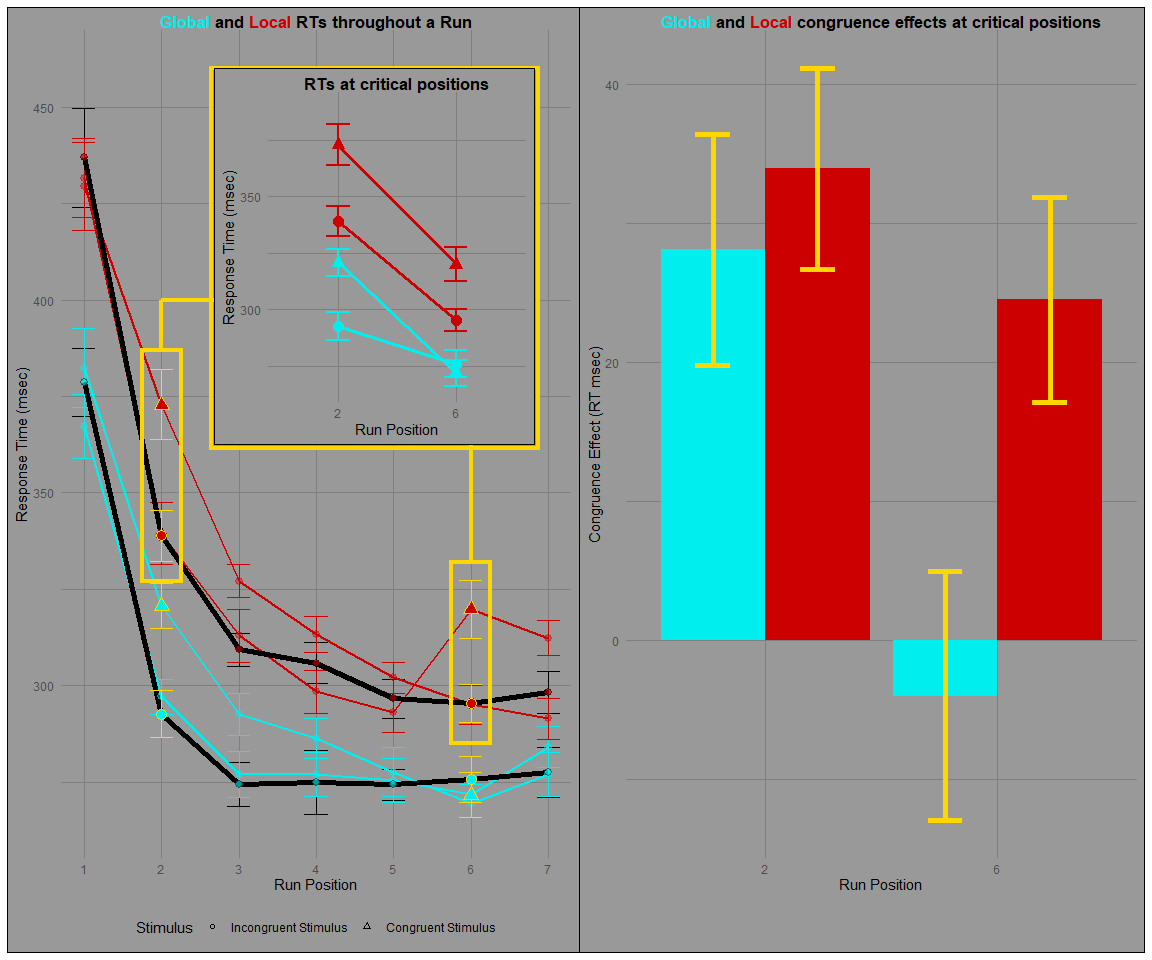
\includegraphics{final_complete_files/figure-latex/all graphs-1.pdf}

\end{document}
